% Homework report template for courses lectured by Blaz Zupan.
% For more on LaTeX please consult its documentation pages, or
% read tutorials like http://tobi.oetiker.ch/lshort/lshort.pdf.
%
% Use pdflatex to produce a PDF of a report.

\documentclass[a4paper,11pt]{article}
\usepackage[slovene]{babel}
\usepackage{a4wide}
\usepackage{fullpage}
\usepackage[toc,page]{appendix}
\usepackage[pdftex]{graphicx} % for figures
\usepackage{setspace}
\usepackage{color}
\definecolor{light-gray}{gray}{0.95}
\usepackage{listings} % for inclusion of Python code
%\usepackage[colorlinks=false]{hyperref}
%\usepackage[hidelinks]{hyperref}
%\usepackage{hyperref}
\usepackage[bookmarks=true,pdfborder={0 0 0}]{hyperref}
\renewcommand{\baselinestretch}{1.2}

\setlength{\parindent}{0pt}

\lstset{ % style for Python code, improve if needed
    language=Python,
    basicstyle=\footnotesize,
    basicstyle=\ttfamily\footnotesize\setstretch{1},
    backgroundcolor=\color{light-gray},
}

\title{Modeliranje brez\v{z}i\v{c}nih omre\v{z}ij}
\author{
    Maja Podbevšek\\
    Peter Benko (63090004)\\
    \v{Z}iga Ham\\
    Miha Zidar (63060317)
}
\date{\today}

\begin{document}

\maketitle

\pagebreak

\tableofcontents

\pagebreak

\section{Zgledi}

\subsection{HandOver}

\subsection{MultiRadio}

\subsection{Synchronized}


\section{Lan80211}



\subsection{Gradniki}

\subsubsection{Access Point}
\label{description:acceesspoint}

slika \ref{image:radio}

opis \ref{description:notificationBoard}

aa

\paragraph{notificationBoard}
\label{description:notificationBoard}

\paragraph{wlan[]}
\label{description:wlan}


\begin{figure}[htbp]
    \begin{center}
        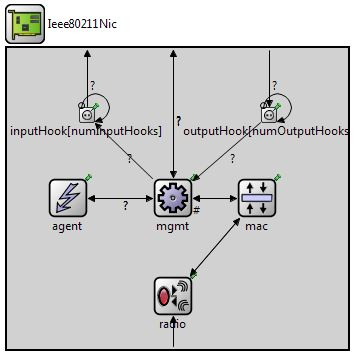
\includegraphics[scale=0.8]{img/radio.jpg}
        \caption{Shema dostopne točke}
	\label{image:radio}
    \end{center}
\end{figure}


\paragraph{relayUnit}
\label{description:relayUnit}


\paragraph{eth[]}
\label{description:eth}


\end{document}

